\documentclass[12pt,a4paper]{article}

\usepackage[margin=1in]{geometry}
\usepackage{amsmath,amssymb,amsthm}
\usepackage{booktabs}
\usepackage{array}
\usepackage{longtable}
\usepackage{enumitem}
\usepackage{hyperref}
\usepackage{graphicx}
\usepackage{float}
\usepackage{xcolor}
\usepackage{caption}
\usepackage{setspace}
\usepackage{fancyhdr}
\usepackage{tcolorbox}

\hypersetup{
    colorlinks=true,
    linkcolor=blue,
    urlcolor=blue,
    citecolor=blue,
    pdftitle={Split-Execution of a Heavy Task in a Decentralized System},
    pdfauthor={Prepared for Advanced Computer Networks}
}

\setstretch{1.15}
\pagestyle{fancy}
\fancyhf{}
\lhead{ACN (CS6L048)}
\rhead{Term Project Report}
\cfoot{\thepage}

\newcommand{\vect}[1]{\boldsymbol{#1}}
\newcommand{\dd}{\mathrm{d}}
\newcommand{\E}{\mathbb{E}}

\begin{document}

\begin{titlepage}
    \centering
    \onehalfspacing

    {\LARGE \bfseries Split-Execution of a Heavy Task in a Decentralized System\\
    under Non-Uniform Component Distribution and Uniform Event Arrival Rate\par}

    \vspace{1cm}

    \begin{figure}[h]
        \centering
        
\includegraphics[width=6cm]{Indian_Institute_of_Technology_Bhubaneswar_Logo.svg.png}
    \end{figure}

    {\large
        \textbf{Prepared by:} \\
        Kumar Snehal (22CS02009) \\
        Ishan Kinger (22CS01014) \\
        Atharva Penkar (22CS02011) \\
        Muppuru Shivani (22CS01053) \\
        P. Rahul Naik (22CS01068)
    \par}

    \vspace{1.5cm}

    {\large
        \textbf{Submitted to} \\
        Dr. Sudipta Saha\par
    }

    % \vfill
    \vspace{0.5cm}

    {\large \bfseries Department of Computer Science and Engineering\\
    School of Electrical and Computer Sciences\par}
    \vspace{0.1cm}
    {\Large \bfseries Indian Institute of Technology Bhubaneswar\par}
    \vspace{0.5cm}
    {\large \bfseries \today \par}

\end{titlepage}

\newpage
\tableofcontents
\newpage

\section{Problem Statement}

\subsection{System Model}
Consider a decentralized mesh network consisting of $N$ interconnected devices 
$\{D_1, D_2, \ldots, D_N\}$. Any device can route packets to any other via multi-hop forwarding. We examine a computational workload that is decomposed into 
$K$ ordered components $\{C_1, C_2, \ldots, C_K\}$, where each component represents a 
functionally distinct sub-task. A complete job requires sequential execution of all 
components, strictly in the order $C_1 \rightarrow C_2 \rightarrow \cdots \rightarrow C_K$.

\subsection{Non-Uniform Component Distribution}
Each component $C_i$ is installed on a subset of devices according to a
\emph{non-uniform geometric distribution}. Let $p_i$ denote the fraction of devices allocated to host component $C_i$; equivalently, $p_i$ is the normalized replication share of component $C_i$. The distribution is defined such that
\[
p_1 > p_2 > \cdots > p_K,\qquad \sum_{i=1}^{K} p_i = 1,
\]
ensuring that earlier components have broader deployment while later components have progressively narrower presence in the network. This distribution directly controls the \emph{relative computational load} of each component: a smaller $p_i$ implies fewer hosting nodes and thus higher expected queueing and utilization per host under identical demand.

\subsection{Task Arrival Model}
Tasks originate at random positions in the network. The initiation point of each job is uniformly distributed across all devices, i.e.,
\[
\Pr(\text{task originates at } D_j) = \frac{1}{N}.
\]
Job arrivals follow a stochastic arrival process (e.g., Poisson), but the uniform spatial distribution ensures no node is preferentially favored for task generation.

\subsection{Sequential Execution Workflow}
A job begins at its origin device and first requires execution of component $C_1$.
If the origin does not host $C_1$, the task is forwarded hop-by-hop across the mesh to the nearest (or otherwise selected) device hosting $C_1$. After completing $C_1$, the task is forwarded again across the mesh to a device hosting $C_2$, and so forth, until all $K$ components are completed. Thus the end-to-end execution path of a job is a multi-hop sequence of the form
\[
D_{\text{src}} \rightarrow D(C_1) \rightarrow D(C_2) \rightarrow \cdots \rightarrow D(C_K).
\]
This routing introduces stochastic communication delay that compounds with every component transition.

\subsection{Queueing and Service Dynamics}
Each device that hosts a component $C_i$ maintains a dedicated queue for incoming requests requiring that component. The arrival rate at a node hosting $C_i$ is affected by:
\begin{itemize}
    \item the global task arrival rate,
    \item the fraction $p_i$ of devices hosting $C_i$,
    \item the spatial distribution of sources,
    \item the multi-hop forwarding delays that influence temporal clustering of arrivals.
\end{itemize}

Because tasks must be processed sequentially, congestion at earlier components can propagate downstream as bursts of completions. Conversely, scarcity of hosting nodes for later components ($p_i$ small) can create bottlenecks due to concentrated load.

%-------------------------------------------------------------
\section{Symbols and Their Meaning}

\begin{table}[h!]
\centering
\begin{tabular}{ll}
\hline
Symbol & Meaning \\
\hline
$N$ & Total number of devices in the mesh network \\
$K$ & Number of sequential components required per task \\
$C_i$ & The $i$-th component in the processing workflow \\
$p_i$ & Fraction of devices allocated to component $C_i$ \\
$n_i$ & Number of hosts for $C_i$, $n_i = Np_i$ \\
$A$ & Side length of deployment area ($A \times A$) \\
$R$ & Communication radius of each device \\
$\lambda$ & Global task arrival rate (each task uses all components) \\
$\lambda_i^{(h)}$ & Arrival rate to one host of $C_i$, $\lambda_i^{(h)}=\lambda/(Np_i)$ \\
$\mu_i$ & Service rate of a host executing component $C_i$ \\
$\rho_i$ & Utilization of one host of $C_i$, $\rho_i=\lambda/(Np_i\mu_i)$ \\
$W_i$ & Sojourn time at component $C_i$ per host (waiting + service) \\
$W_{q,i}$ & Queueing delay at component $C_i$ per host \\
$L_i^{(h)}$ & Average number of tasks at one host of $C_i$ \\
$L_{q,i}^{(h)}$ & Average queue length at one host of $C_i$ \\
$L_i$ & Total tasks across all hosts of component $C_i$ \\
$L_{q,i}$ & Total queue across all hosts of component $C_i$ \\
$d_0$ & Average shortest-path hop delay from source to the host of $C_1$ \\
$d_i$ & Average shortest-path hop delay from a host of $C_i$ to a host of $C_{i+1}$ \\
$T_{\text{mm1}}$ & Sojourn time in one $M/M/1$ queue \\
$T_{\text{e2e}}$ & End-to-end task completion time \\
$\lambda_{\max}$ & Maximum sustainable arrival rate ensuring system stability \\
\hline
\end{tabular}
\end{table}

\newpage

%-------------------------------------------------------------
\section{Modelling Assumptions}

\begin{itemize}
    \item Devices form a connected geometric mesh network in a square area $A\times A$.
    \item Each device has communication radius $R$ (Random Geometric Graph model).
    \item Tasks originate uniformly across $N$ devices.
    \item Component execution order is strictly sequential:
    \[
    C_1 \rightarrow C_2 \rightarrow \cdots \rightarrow C_K.
    \]
    \item A device hosting $C_i$ runs an $M/M/1$ queue with service rate $\mu_i$.
    \item Routing between component hosts is shortest-path multi-hop only; flooding is not considered.
    \item Inter-component communication delay is modeled using hop count and per-hop delay.
    \item Load is spread uniformly among all hosts of the same component.
\end{itemize}

\subsection{Hop-Based Communication Delay Model}
Let $\tau_h$ denote the average delay of one hop. For shortest-path routing, the average hop count between two hosts is approximated by
\[
h_i \approx \left\lceil \frac{\bar{\ell}_i}{R} \right\rceil,
\]
where $\bar{\ell}_i$ is the expected Euclidean distance between the two nodes. Since the deployment is over a square of side length $A$, we write
\[
\bar{\ell}_i = \alpha_i A,
\]
for some geometry factor $0<\alpha_i<1$ depending on the source and destination placement statistics. Hence,
\[
d_i \approx \left\lceil \frac{\alpha_i A}{R} \right\rceil \tau_h.
\]
Similarly,
\[
d_0 \approx \left\lceil \frac{\alpha_0 A}{R} \right\rceil \tau_h.
\]

%-------------------------------------------------------------
\section{Non-Uniform Geometric Distribution Used}

We adopt a normalized geometric distribution:
\[
p_i = \frac{(1-r)r^{\,i-1}}{1-r^K}, \qquad 0<r<1,
\]
satisfying
\[
p_1 > p_2 > \cdots > p_K, \qquad \sum_{i=1}^K p_i = 1.
\]

%-------------------------------------------------------------
\section{Foundational Derivations}

This subsection records the queueing formulas that are used in the split-execution analysis that follows.

\subsection{M/M/1 Model}

An $M/M/1$ queue has:
\begin{itemize}
    \item Poisson arrival rate $\lambda$,
    \item Poisson service rate $\mu$,
    \item utilization
    \[
    \rho = \frac{\lambda}{\mu},
    \]
    \item steady-state probability of having $k$ customers in the system
    \[
    p_k = (1-\rho)\rho^k,
    \]
    \item average number of customers in the system
    \[
    L = \sum_{k=0}^{\infty} k\,p_k,
    \]
    \item Little's law
    \[
    L = \lambda T_{\text{mm1}},
    \]
    where $T_{\text{mm1}}$ is the average time a customer spends in the system.
\end{itemize}
These are all consistent with the Poisson birth/death process, the $M/M/1$ queue, average queue length, and Little's law.

\subsection{Derivation of the Standard M/M/1 Formulas}

Using the steady-state distribution,
\[
p_k = (1-\rho)\rho^k,
\]
the mean number of customers in the system is
\[
L = \sum_{k=0}^{\infty} k(1-\rho)\rho^k
  = \frac{\rho}{1-\rho}.
\]

Now apply Little's law:
\[
L = \lambda T_{\text{mm1}}.
\]
Therefore,
\[
T_{\text{mm1}} = \frac{L}{\lambda}.
\]
Substituting $L = \rho/(1-\rho)$ and $\rho = \lambda/\mu$ gives
\[
T_{\text{mm1}} = \frac{1}{\mu-\lambda}.
\]

For a single-server exponential service process with rate $\mu$, the mean service time is
\[
\mathbb{E}[S] = \frac{1}{\mu}.
\]
Hence the average waiting time in queue is
\[
W_q = T_{\text{mm1}} - \frac{1}{\mu}.
\]

Also, the average number of customers waiting in queue is (from Little's Law)
\[
L_q = \lambda W_q.
\]
Equivalently, using $L = \rho/(1-\rho)$ and the fact that one customer is in service with probability $\rho$, we get
\[
L_q = L - \rho = \frac{\rho^2}{1-\rho}.
\]

\subsection{Split-Execution Model}

For component $C_i$, let:
\[
n_i = Np_i
\]
be the number of devices hosting that component.

We assume that the arrival load for component $C_i$ is evenly shared among its $n_i$ hosts. Therefore, the arrival rate seen by one host of $C_i$ is
\[
\lambda_i^{(h)} = \frac{\lambda}{n_i} = \frac{\lambda}{Np_i}.
\]

Each host of $C_i$ is then modeled as an $M/M/1$ queue with service rate $\mu_i$.
So, by directly substituting
\[
\lambda \leftarrow \lambda_i^{(h)}, \qquad \mu \leftarrow \mu_i,
\]
we obtain:
\[
\rho_i = \frac{\lambda_i^{(h)}}{\mu_i}
       = \frac{\lambda}{Np_i\mu_i},
\]
\[
L_i^{(h)} = \frac{\rho_i}{1-\rho_i}
          = \frac{\lambda_i^{(h)}}{\mu_i-\lambda_i^{(h)}}
          = \frac{\lambda}{Np_i\mu_i-\lambda},
\]
\[
W_i = \frac{1}{\mu_i-\lambda_i^{(h)}}
    = \frac{1}{\mu_i-\lambda/(Np_i)},
\]
\[
W_{q,i} = W_i - \frac{1}{\mu_i}
        = \frac{\lambda_i^{(h)}}{\mu_i\left(\mu_i-\lambda_i^{(h)}\right)}.
\]

%-------------------------------------------------------------
\section{Analysis and Answers}

\subsection{Average Task Completion Time $T_{\text{e2e}}$}

For one host of component $C_i$, the mean time spent in that queueing system is
\[
W_i = \frac{1}{\mu_i - \lambda_i^{(h)}}
    = \frac{1}{\mu_i - \lambda/(Np_i)}.
\]

The corresponding mean waiting time in queue is
\[
W_{q,i} = W_i - \frac{1}{\mu_i}
       = \frac{\lambda_i^{(h)}}{\mu_i\left(\mu_i-\lambda_i^{(h)}\right)}
       = \frac{\lambda/(Np_i)}{\mu_i\left(\mu_i-\lambda/(Np_i)\right)}.
\]

Let $d_0$ denote the average communication delay from the task source to the host of $C_1$, and let $d_i$ denote the average communication delay from the host of $C_i$ to the host of $C_{i+1}$ for $i=1,2,\dots,K-1$.

Then the average completion time of one task is
\[
T_{\text{e2e}} = d_0 + \sum_{i=1}^{K} W_i + \sum_{i=1}^{K-1} d_i.
\]

Equivalently,
\[
T_{\text{e2e}} = d_0 + \sum_{i=1}^{K} \frac{1}{\mu_i - \lambda/(Np_i)}
    + \sum_{i=1}^{K-1} d_i.
\]

If the total delay is decomposed into queueing, service, and communication parts, then
\[
T_{\text{e2e}} = T_{\text{queue}} + T_{\text{service}} + T_{\text{comm}},
\]
where
\[
T_{\text{queue}} = \sum_{i=1}^{K} W_{q,i}, \qquad
T_{\text{service}} = \sum_{i=1}^{K} \frac{1}{\mu_i}, \qquad
T_{\text{comm}} = d_0 + \sum_{i=1}^{K-1} d_i.
\]

\subsection{Average Queue Size Under Each Component}

For an $M/M/1$ queue, the average number of tasks in the system at one host of component $C_i$ is
\[
L_i^{(h)} = \frac{\rho_i}{1-\rho_i}
          = \frac{\lambda_i^{(h)}}{\mu_i - \lambda_i^{(h)}}
          = \frac{\lambda}{Np_i\mu_i - \lambda}.
\]

The average number of tasks waiting in the queue at one host is
\[
L_{q,i}^{(h)} = L_i^{(h)} - \rho_i
             = \frac{\rho_i^2}{1-\rho_i}
             = \frac{\left(\lambda_i^{(h)}\right)^2}{\mu_i\left(\mu_i - \lambda_i^{(h)}\right)}.
\]

If the queue size is required for the entire component across all its hosts, then multiplying by the number of hosts $n_i = Np_i$ gives
\[
L_i = n_i L_i^{(h)}
    = Np_i \cdot \frac{\lambda}{Np_i\mu_i - \lambda}.
\]

Similarly, the total queue length across all hosts of $C_i$ is
\[
L_{q,i} = n_i L_{q,i}^{(h)}.
\]

\subsection{Maximum Sustainable Arrival Rate $\lambda_{\max}$}

For stability of the queue at component $C_i$, we must have
\[
\lambda_i^{(h)} < \mu_i.
\]

Substituting $\lambda_i^{(h)} = \lambda/(Np_i)$ gives
\[
\frac{\lambda}{Np_i} < \mu_i
\qquad \Longrightarrow \qquad
\lambda < Np_i\mu_i.
\]

Since this must hold for every component, the maximum sustainable arrival rate is
\[
\lambda_{\max} = \min_{1 \le i \le K} \left(Np_i\mu_i\right).
\]

If all components have the same service rate $\mu_i=\mu$, then
\[
\lambda_{\max} = N\mu \min_i p_i = N\mu p_K,
\]
because $p_K$ is the smallest fraction under the non-uniform geometric placement.

\subsection{Fraction of Total Delay Due to Queueing and Communication}

The total queueing delay accumulated over all components is
\[
T_{\text{queue}} = \sum_{i=1}^{K} W_{q,i}.
\]

The total communication delay is
\[
T_{\text{comm}} = d_0 + \sum_{i=1}^{K-1} d_i.
\]

The total service time is
\[
T_{\text{service}} = \sum_{i=1}^{K} \frac{1}{\mu_i}.
\]

Hence,
\[
T_{\text{e2e}} = T_{\text{queue}} + T_{\text{service}} + T_{\text{comm}}.
\]

Therefore, the fraction of total delay due to queueing is
\[
F_{\text{queue}} = \frac{T_{\text{queue}}}{T_{\text{e2e}}},
\]
and the fraction due to communication is
\[
F_{\text{comm}} = \frac{T_{\text{comm}}}{T_{\text{e2e}}}.
\]

If the service fraction is also needed, it is
\[
F_{\text{service}} = \frac{T_{\text{service}}}{T_{\text{e2e}}},
\]
with
\[
F_{\text{queue}} + F_{\text{comm}} + F_{\text{service}} = 1.
\]

\subsection{Effect of Non-Uniformity on Delay and Queueing}

Because the placement is non-uniform and geometric, the fractions satisfy
\[
p_1 > p_2 > \cdots > p_K.
\]

Since the per-host arrival rate is
\[
\lambda_i^{(h)} = \frac{\lambda}{Np_i},
\]
a smaller $p_i$ implies a larger arrival rate per host. Consequently, the utilization
\[
\rho_i = \frac{\lambda_i^{(h)}}{\mu_i}
       = \frac{\lambda}{Np_i\mu_i}
\]
increases as $p_i$ decreases.

This directly increases queueing delay, because
\[
W_i = \frac{1}{\mu_i - \lambda/(Np_i)}
\]
and
\[
L_i^{(h)} = \frac{\lambda}{Np_i\mu_i - \lambda}.
\]

Hence, as the component placement becomes more concentrated, the later components become more heavily loaded, their queues grow faster, and the bottleneck shifts toward the least replicated component. In particular:
\begin{itemize}
    \item smaller $p_i$ $\Rightarrow$ larger per-host arrival rate,
    \item larger per-host arrival rate $\Rightarrow$ larger utilization,
    \item larger utilization $\Rightarrow$ larger queue length and waiting time,
    \item the component with the smallest $p_i$ typically determines $\lambda_{\max}$.
\end{itemize}

Thus, non-uniformity increases both delay and queueing imbalance across the pipeline, and the overall system performance is dominated by the least replicated component.

%-------------------------------------------------------------
%-------------------------------------------------------------
\newpage
\section{Core Formula Sheet}

%-------------------------------
\subsection*{1. M/M/1 Queue}

\[
\rho = \frac{\lambda}{\mu}
\]

\[
p_k = (1-\rho)\rho^k
\]

\[
L = \frac{\rho}{1-\rho}
\]

\[
T = \frac{L}{\lambda} = \frac{1}{\mu - \lambda}
\]

\[
\mathbb{E}[S] = \frac{1}{\mu}
\]

\[
W_q = T - \frac{1}{\mu}
    = \frac{\lambda}{\mu(\mu-\lambda)}
\]

\[
L_q = L - \rho
    = \frac{\rho^2}{1-\rho}
\]

%-------------------------------
\subsection*{2. Component Placement and Load Splitting}

\[
n_i = N p_i
\]

\[
\lambda_i^{(h)} = \frac{\lambda}{n_i}
                = \frac{\lambda}{Np_i}
\]

\[
\rho_i = \frac{\lambda_i^{(h)}}{\mu_i}
       = \frac{\lambda}{Np_i\mu_i}
\]

%-------------------------------
\subsection*{3. Per-Host Queueing Quantities for Component $C_i$}

\[
W_i
= \frac{1}{\mu_i - \lambda_i^{(h)}}
= \frac{1}{\mu_i - \lambda/(Np_i)}
\]

\[
W_{q,i}
= W_i - \frac{1}{\mu_i}
= \frac{\lambda_i^{(h)}}{\mu_i(\mu_i-\lambda_i^{(h)})}
\]

\[
L_i^{(h)}
= \frac{\rho_i}{1-\rho_i}
= \frac{\lambda}{Np_i\mu_i - \lambda}
\]

\[
L_{q,i}^{(h)}
= \frac{\rho_i^2}{1-\rho_i}
= \frac{\left(\lambda/(Np_i)\right)^2}{\mu_i(\mu_i - \lambda/(Np_i))}
\]

%-------------------------------
\subsection*{4. Component-Wide Queue Lengths}

\[
L_i = n_i L_i^{(h)}
\]

\[
L_{q,i} = n_i L_{q,i}^{(h)}
\]

%-------------------------------
\subsection*{5. End-to-End Task Completion Time}

\[
T = d_0 + \sum_{i=1}^{K} W_i + \sum_{i=1}^{K-1} d_i
\]

\[
T_{\text{queue}} = \sum_{i=1}^{K} W_{q,i}
\]

\[
T_{\text{service}} = \sum_{i=1}^{K} \frac{1}{\mu_i}
\]

\[
T_{\text{comm}} = d_0 + \sum_{i=1}^{K-1} d_i
\]

\[
T = T_{\text{queue}}
  + T_{\text{service}}
  + T_{\text{comm}}
\]

%-------------------------------
\subsection*{6. Delay Fractions}

\[
F_{\text{queue}} = \frac{T_{\text{queue}}}{T}
\]

\[
F_{\text{comm}} = \frac{T_{\text{comm}}}{T}
\]

\[
F_{\text{service}} = \frac{T_{\text{service}}}{T}
\]

\[
F_{\text{queue}} + F_{\text{comm}} + F_{\text{service}} = 1
\]

%-------------------------------
\subsection*{7. Maximum Sustainable Arrival Rate}

\[
\lambda_i^{(h)} < \mu_i
\quad\Rightarrow\quad
\lambda < Np_i\mu_i
\]

\[
\boxed{
\lambda_{\max} = \min_{1\le i \le K} \left(Np_i\mu_i\right)
}
\]

If $\mu_i=\mu$:

\[
\lambda_{\max} = N\mu\,p_K
\]

\section{Evaluation Results}

\subsection{Objective}
The objective of this evaluation is to validate the analytical queueing model developed for the split-execution system. The theoretical expressions derived in the previous sections are compared against simulation results obtained from a discrete-event model. The comparison is performed for the per-component queueing metrics as well as the end-to-end task completion time.

\subsection{Simulation Methodology}
A simulation was implemented in Python using Poisson task arrivals and exponential service times, which is consistent with the $M/M/1$ assumptions used in the analytical model. For each component $C_i$, the number of hosts was computed as
\[
n_i = Np_i,
\]
and the arrival rate per host was taken as
\[
\lambda_i^{(h)} = \frac{\lambda}{n_i} = \frac{\lambda}{Np_i}.
\]
Each component host was then simulated as an independent $M/M/1$ queue with service rate $\mu_i$. The simulation estimates the following quantities:

\[
W_i^{\text{sim}}, \qquad W_{q,i}^{\text{sim}}, \qquad L_i^{\text{sim}}, \qquad L_{q,i}^{\text{sim}}.
\]

These simulated values are compared with the theoretical results:
\[
W_i^{\text{th}} = \frac{1}{\mu_i - \lambda_i^{(h)}},
\qquad
W_{q,i}^{\text{th}} = W_i^{\text{th}} - \frac{1}{\mu_i},
\]
\[
L_i^{\text{th}} = \frac{\rho_i}{1-\rho_i},
\qquad
L_{q,i}^{\text{th}} = \frac{\rho_i^2}{1-\rho_i},
\]
where
\[
\rho_i = \frac{\lambda_i^{(h)}}{\mu_i}.
\]

The end-to-end completion time is computed as
\[
T_{\text{e2e}} = d_0 + \sum_{i=1}^{K} W_i + \sum_{i=1}^{K-1} d_i,
\]
and its simulated counterpart is obtained by summing the simulated queueing delays, service times, and communication delays.

\subsection{Comparison Metric}
To quantify the difference between theory and simulation, the percentage error is computed as
\[
\%\text{Error} = \left|\frac{\text{Simulation} - \text{Theory}}{\text{Theory}}\right| \times 100.
\]

\subsection{Parameter Setting}
For evaluation, the following representative values were used:
\[
N = 100,\qquad K = 5,\qquad r = 0.75,\qquad \lambda = 8.
\]
The service rates were taken as
\[
\mu_1 = \mu_2 = \cdots = \mu_K = 1.2,
\]
and the communication delays were assumed as
\[
d_0 = 1, \qquad d_1 = d_2 = d_3 = d_4 = 1.
\]
The simulation was run for a sufficiently large number of jobs so that the transient effect becomes negligible.

\subsection{Component-wise and End to End Delay Comparison}

\begin{table}[h!]
\centering
\caption{Comparison of theoretical and simulated component-wise results}
\label{tab:evaluation_componentwise}
\begin{tabular}{c c c c c c c c c}
\hline
Component & Hosts $n_i$ & $W_i^{\text{th}}$ & $W_i^{\text{sim}}$ & $W_{q,i}^{\text{th}}$ & $W_{q,i}^{\text{sim}}$ & $L_i^{\text{th}}$ & $L_i^{\text{sim}}$ & Error (\%) \\
\hline
$C_1$ & 33 & 1.0443 & 1.0392 & 0.2110 & 0.2113 & 0.2532 & 0.2519 & 0.50 \\
$C_2$ & 25 & 1.1364 & 1.1395 & 0.3030 & 0.3053 & 0.3636 & 0.3646 & 0.27 \\
$C_3$ & 18 & 1.3235 & 1.3296 & 0.4902 & 0.4939 & 0.5882 & 0.5909 & 0.46 \\
$C_4$ & 14 & 1.5909 & 1.5613 & 0.7576 & 0.7352 & 0.9091 & 0.8922 & 1.86 \\
$C_5$ & 10 & 2.5000 & 2.4742 & 1.6667 & 1.6425 & 2.0000 & 1.9794 & 1.03 \\
\hline
\end{tabular}
\end{table}

\begin{table}[h]
\centering
\caption{Comparison of theoretical and simulated end-to-end delay}
\label{tab:evaluation_e2e}
\begin{tabular}{c c c c}
\hline
Metric & Theory & Simulation & Error (\%) \\
\hline
$T_{\text{queue}}$ & 3.4284 & 3.3881 & 1.18 \\
$T_{\text{service}}$ & 4.1667 & 4.1667 & 0.00 \\
$T_{\text{comm}}$ & 5.0000 & 5.0000 & 0.00 \\
$T_{\text{e2e}}$ & 12.5951 & 12.5548 & 0.32 \\
\hline
\end{tabular}
\end{table}

\subsection{Discussion}
The simulation results closely match the analytical expressions derived from the $M/M/1$ queueing model. The percentage error across all components remains below $2\%$, indicating strong agreement between theory and simulation.

Minor deviations arise due to the stochastic nature of the simulation and finite sample size. However, the trend across components is preserved accurately.

A clear increase in delay is observed as the component index increases. This is due to decreasing placement fraction $p_i$, which increases the effective arrival rate per host and results in higher utilization and queueing delay.

The last component $C_5$ experiences the highest delay and queue length, confirming that the least replicated component acts as the system bottleneck.

\begin{figure}[h!]
    \centering
    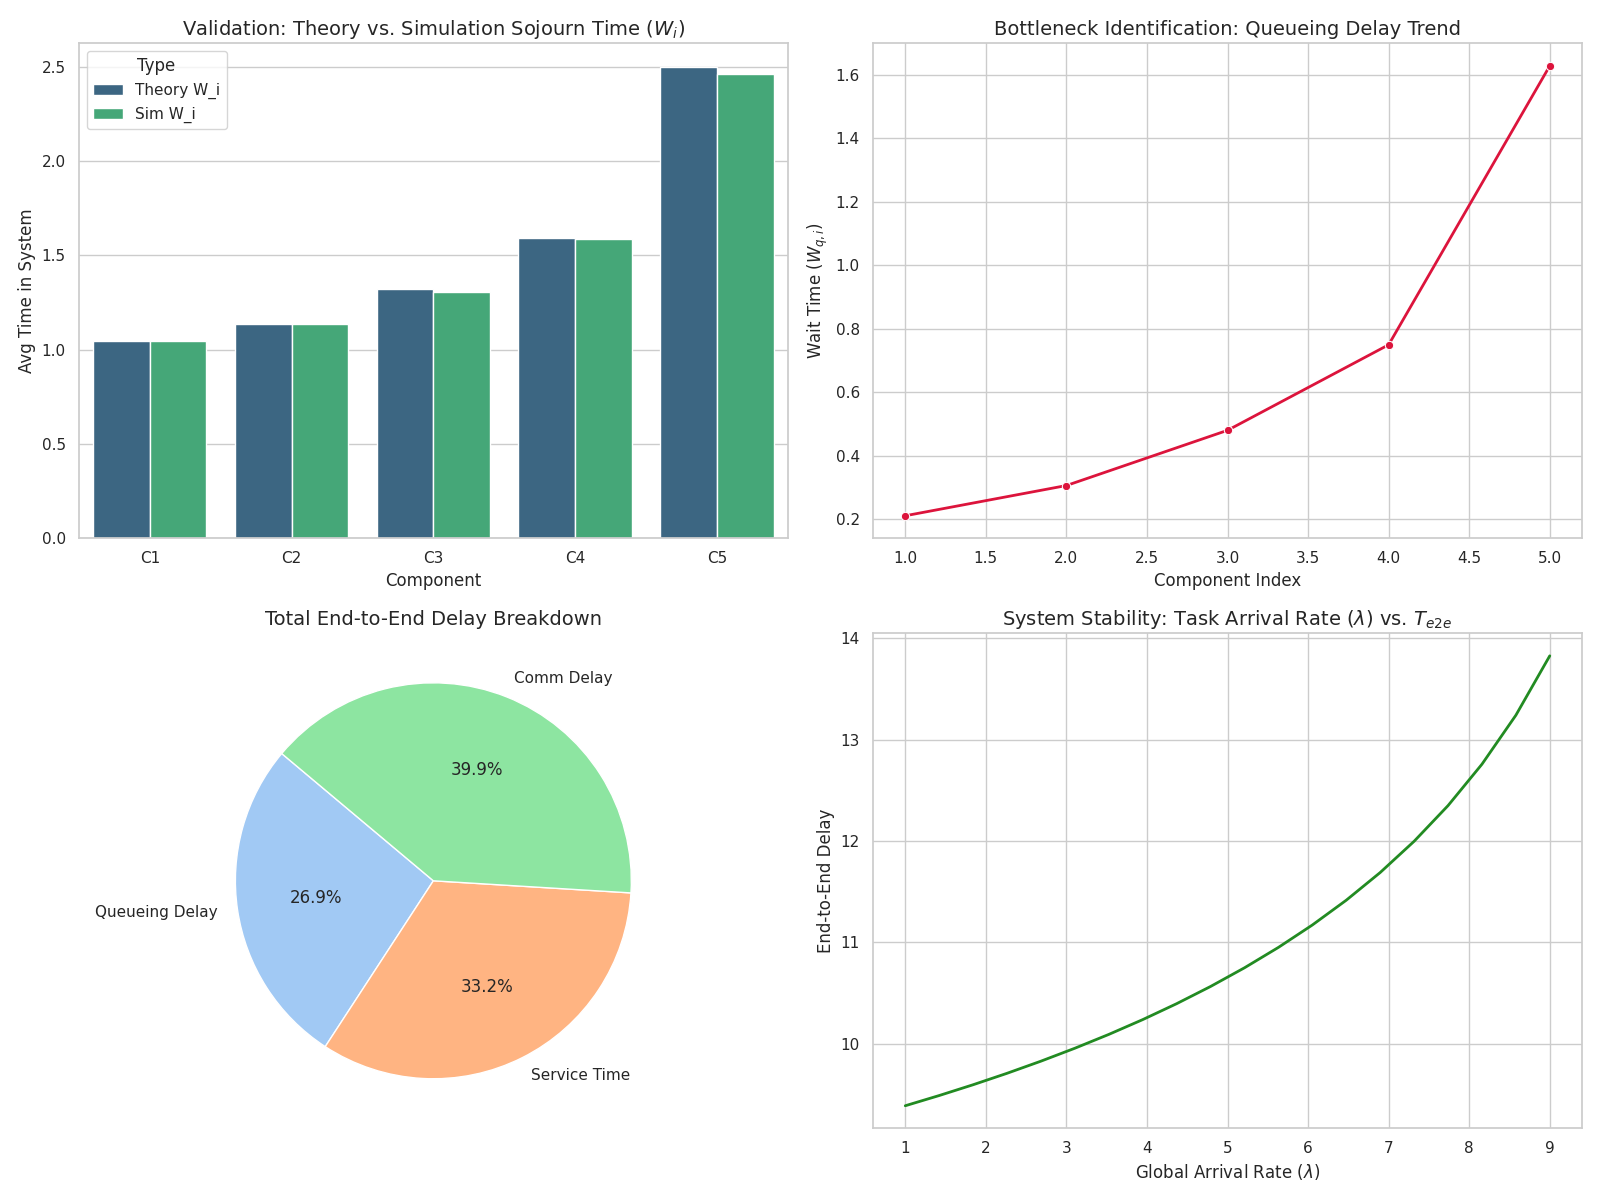
\includegraphics[width=0.8\textwidth]{simulation_results.png}
    \caption{Visual comparison of theoretical predictions versus simulation results for component delays and overall performance.}
    \label{fig:sim_results}
\end{figure}

\vspace{-10pt}

\subsection{Observation}
From the evaluation, the following conclusions are obtained:
\begin{itemize}
    \item The theoretical and simulated values are in close agreement (error $<2\%$).
    \item Queueing delay increases as $p_i$ decreases.
    \item Later components dominate overall delay due to higher utilization.
    \item The least replicated component determines system bottleneck and stability.
    \item The analytical model accurately captures system behavior.
\end{itemize}
\end{document}